\documentclass{article}

\usepackage[a4paper, hmargin={20mm, 20mm}, vmargin={25mm, 30mm}]{geometry}
\usepackage[utf8]{inputenc}
\usepackage[english, main=portuguese]{babel}

\usepackage[hidelinks]{hyperref}
\usepackage{bookmark}
\usepackage{cancel}
\usepackage{comment}

\usepackage{array}
\usepackage{indentfirst}
\usepackage{multicol}
\usepackage{subfiles}

\usepackage{amsmath}
\usepackage{amssymb}
\usepackage{systeme}
\usepackage{float}
\usepackage{enumitem}
\restylefloat{table}

\usepackage{graphicx}
\graphicspath{ {./IMAGENS/} }

% Pacote para a definição de novas cores
\usepackage{xcolor}
% Definindo novas cores
\definecolor{darkgreen}{rgb}{0.0, 0.42, 0.24}
\definecolor{darkpurple}{rgb}{0.74, 0.2, 0.64}
\definecolor{darkblue}{rgb}{0.0, 0.28, 0.67}

% Configurando layout para mostrar codigos Java
\usepackage{listings}


\newcommand{\myStyle}{
\lstset{
    language=Octave,                            % the language of the code
    basicstyle=\ttfamily\small,               % the size of the fonts that are used for the code
    keywordstyle=\color{darkpurple}\bfseries, %
    stringstyle=\color{darkblue},             %
    commentstyle=\color{darkgreen},           %
    morecomment=[s][\color{blue}]{/**}{*/},   %
    extendedchars=true,                       %
    showtabs=false,                           % show tabs within strings adding particular underscores
    showspaces=false,                         % show spaces adding particular underscores
    showstringspaces=false,                   % underline spaces within strings
    numbers=left,                             % where to put the line-numbers
    numberstyle=\tiny\color{gray},            % the style that is used for the line-numbers
    stepnumber=1,                             % the step between two line-numbers. If it's 1, each line will be numbered
    numbersep=5pt,                            % how far the line-numbers are from the code
    frame=single,                             % adds a frame around the code
    rulecolor=\color{black},                  % if not set, the frame-color may be changed on line-breaks within not-black text
    breaklines=true,                          % sets automatic line breaking
    backgroundcolor=\color{white},            % choose the background color
    breakatwhitespace=true,                   % sets if automatic breaks should only happen at whitespace
    breakautoindent=false,                    %
    captionpos=b,                             % sets the caption-position to bottom
    xleftmargin=0pt,                          %
    tabsize=2,                                % sets default tabsize to 2 spaces
}}


\begin{document}
    \begin{titlepage}
        \begin{center}
            \rule{450pt}{0.5pt}\\[4mm]
            {\Huge MS211 - Cálculo Numérico}\\
            \rule{450pt}{0.5pt}\\[2mm]
            {\Large Laboratório 07}\\[200mm]
            \today\\
            \rule{250pt}{0.5pt}\\
            {\large Guilherme Nunes Trofino}\\
            {\large 217276}\\
        \end{center}
    \end{titlepage}
\newpage

    \section{Questão}
        \subsection{Introdução}
            \paragraph{Problema}Notou-se que o exército de Leônidas I era composto por $M$ guerreiros espartanos, cuja distribuição $N(h)$ das alturas pode ser representada pela seguinte equação de distribuição normal:
                \begin{equation}
                    N(h) = \frac{M}{\sigma\sqrt{2\pi}} \cdot e^{-\frac{(h - \mu)^{2}}{2\sigma^2}}
                \end{equation}
            Onde:
                \begin{enumerate}[noitemsep]
                    \item $\mu$: Representa a \textbf{Média das Alturas};
                    \item $\sigma$: Representa o \textbf{Desvio Padrão};
                \end{enumerate}
            Assim, pode-se obter quantos guerreiros possuem altura entre $a$ e $b$ integrando a distribuição normal no intervalo desejado como representado na equação:
                \begin{equation}
                    N = \int_{a}^{b} N(h) dh
                \end{equation}

            \paragraph{Determine}Toma-se $M = 300$, $\mu = 1,7m$ e $\sigma = 0,1m$.
                \begin{enumerate}[noitemsep]
                    \item Estime quantos guerreiros possuem altura entre $1,8m$ e $2,0m$?
                    \item Estime o erro cometido na estimativa.
                \end{enumerate}

        \subsection{Desenvolvimento}
            \paragraph{Teoria}Sabe-se do Cálculo I que uma integral definida será formalmente dada, por definição, pela seguinte equação:
                \begin{equation}
                    \boxed{\int_{a}^{b} f(x) dx = \lim_{n\to\infty} \sum_{k=1}^{n} f(x_{k})\cdot\Delta x}
                \end{equation}
            Onde:
                \[\Delta x = \frac{b - a}{n} \text{ e } x_{k} \in [a, b]\]
            Todavia, esta definição pode ser aproximada numericamente através da \textbf{Fórmula de Quadratura}. Desta forma temos a seguinte equação para $n+1$ pontos no intervalo desejado:
                \begin{equation}
                    \boxed{\int_{a}^{b} f(x) dx = \sum_{k=0}^{n} w_{k} \cdot f(x_{k}) + R_{n+1}}
                \end{equation}
                \[\int_{a}^{b} f(x) dx\approx \sum_{k=0}^{n} w_{k} \cdot f(x_{k})\]
            Onde:
                \begin{enumerate}[noitemsep]
                    \item $x_{0}, x_{1}, \dots, x_{n} \in [a, b]$ são \textbf{Nós de Integração};
                    \item $w_{0}, w_{1}, \dots, w_{n}$ são os \textbf{Pesos} dos respectivos nós;
                    \item $R_{n+1}$ será o \textbf{Resto} da aproximação;
                \end{enumerate}

            \paragraph{Fórmula de Newton-Cotes}Aplicam-se interpolações polinomiais nos pontos igualmente espaçados, $x_{0} < x_{1} < \cdots < x_{n}$, do intervalo fechado $[a, b]$. Assim, os pontos podem ser relacionados através de um polinômio interpolador de $f$ no intervalo:
                \[x_{k} = a + \frac{b - a}{n} k, \hspace{2.5mm} \forall k = 0, 1, \dots, n\]

            \paragraph{Regra dos Trapézios Repetidas}Nesta formulação aproxima-se $f$ por um polinômio linear interpolado por partes $\Lambda(x)$ em $x_{0}, x_{1}, \dots, x_{n}$. Nesta abordagem tem-se a seguinte equação:
                \[\int_{a}^{b} f(x) dx = \sum_{k = 1}^{n} \int_{x_{k-1}}^{x_{k}} \Lambda(x) dx\]
                \[\int_{a}^{b} f(x) dx = \sum_{k - 1}^{n} \left(\frac{h}{2}\left(f(x_{k-1}) + f(x_{k})\right) - \frac{h^{3}}{12} f''(\eta_{k})\right)\]
                \begin{equation}
                    \boxed{
                        \int_{a}^{b} f(x) dx = 
                        \underbrace{\frac{h}{2} \sum_{k - 1}^{n} \left(f(x_{k-1}) + f(x_{k})\right)}_{T_{n}(f)}
                        - 
                        \underbrace{\frac{h^{3}}{12} \sum_{k - 1}^{n} f''(\eta_{k})}_{R_{T}}
                    }
                \end{equation}

            \paragraph{Aproximação}Desta maneira, pode-se representar uma aproximação numérica para integral desejada, através dos \textbf{Trapézios Repetidos}, pode ser calculado pela seguinte equação:
                \[\boxed{T_{n}(f) = \frac{h}{2}\left(f(x_{0}) + 2f(x_{1}) + \cdots + 2f(x_{n-1}) + f(x_{n})\right)}\]

            \paragraph{Erro}Desta maneira, pode-se representar uma aproximação numérica para o erro da integral, através dos \textbf{Trapézios Repetidos}, pode ser calculado pelas seguintes equações:
                \[\boxed{R_{T} \leq \frac{b - a}{12} h^{2} M_{2}}\]
            O teorema do valor intermediário garante que, dado $f''$ contínua em $[a, b]$, existe $\epsilon \in (a, b)$ tal que o \textbf{Majorante} seja obtido pela seguinte equação:
                \[M_{2} = \max_{a\leq\epsilon\leq b} |f''(\epsilon)|\]

        \subsection{Solução}
            \paragraph{Método dos Trapézios}A integral de uma função, como apresentado no desenvolvimento, pode ser calculada através do \textbf{Método dos Trapézios Repetidos}. Optou-se por este por sua simplicidade de implementação e compreensão.

            \paragraph{Observação}Considerou-se $n = 300$ intervalos para interação do método, entretanto para o erro dos trapézios repetidos calculou-se a derivada de segunda ordem da função $N(h)$ através do \textbf{WolframAlpha}, obtendo a seguinte equação:
            \[\boxed{f''(x) = 1.19683 \cdot 10^{7} \cdot (x -1.8)\cdot(x -1.6) \cdot e^{-50 \cdot (-1.7 + x)^2}}\]

                \begin{figure}[h]
                    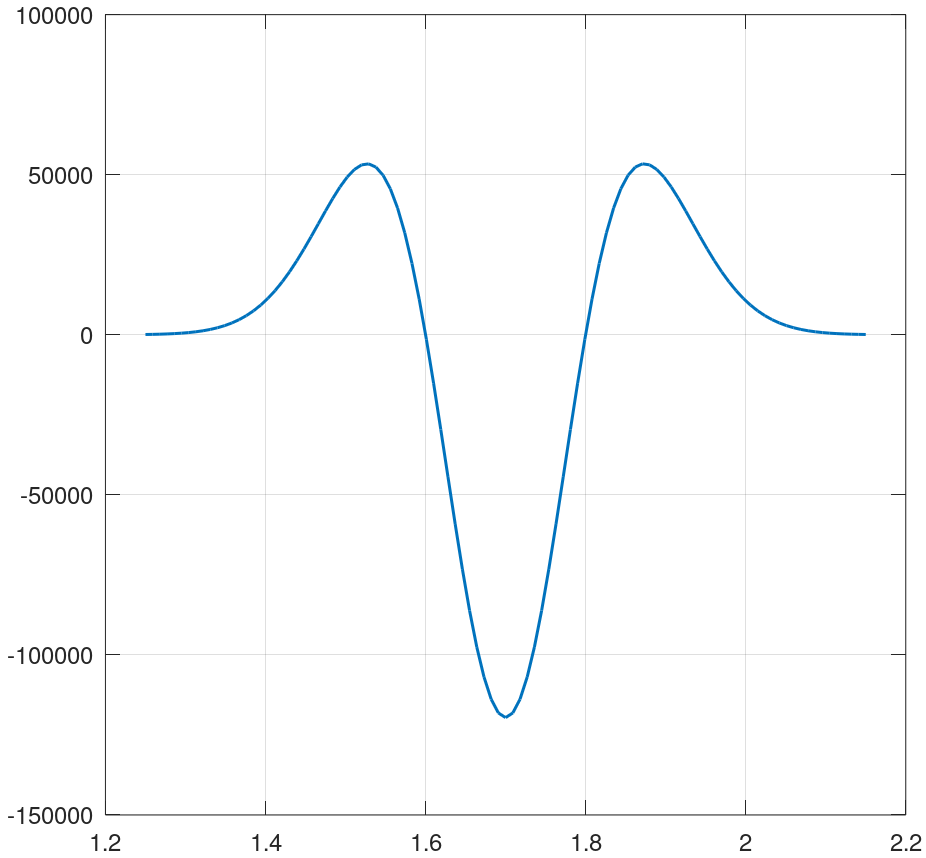
\includegraphics[width = 6cm]{derivada.png}
                    \centering
                \end{figure}
            \paragraph{Análise}A partir do gráfico pode-se concluir que o \textbf{Majorante} $M_{2}$, valor de pico da função, ocorre em $x = 1.7$. Assim pode-se concluir:
            \[\boxed{M_{2} = \max_{a\leq\epsilon\leq b} |f''(1.7)| = 119683}\]

            \paragraph{Aproximação}Desta forma, pelo Método dos Trapézios Repetidos, haveriam $47.19$ guerreiros, aproximadamente $47$, que possuem alturas entre $1,8m$ e $2m$, apresentando aproximadamente $0.0079722$ de erro nesta estimativa.

        \subsection{Códigos}
        \begin{scriptsize}
            \myStyle
            \lstinputlisting{IntegralTrapezioRepetido.m}
            \lstinputlisting{AT7_1.m}
        \end{scriptsize}
\newpage

    \section{Questão}
        \subsection{Introdução}
            \paragraph{Problema}Considera-se a função gamma definida pela seguinte equação:
                \begin{equation}
                    \Gamma (x) = \int_{0}^{\infty} t^{x-1} \cdot e^{-t} dt, \hspace{2.5mm} x>0
                \end{equation}
            Pode-se mostrar, usando integração por partes, que $\Gamma (x) = (x-1) \Gamma (x-1)$ e $\Gamma (1) = 1$, satisfazendo assim $\Gamma (n) = (n-1)!$ para todo natural $n > 0$ como mostrado na tabela:
                \[
                    \begin{array}{c | c c c c c}
                        x         & 1 & 2 & 3 & 4 & 5\\\hline
                        \Gamma(x) & 1 & 1 & 2 & 6 & 24
                    \end{array}
                \]

            \paragraph{Determine}Interpola-se a tabela acima, obtém-se uma aproximação da função $\Gamma$.
                \begin{enumerate}[noitemsep]
                    \item Determine o polinômio de grau 4 que interpola a tabela acima.
                    \item Determine uma spline cúbica que interpola a tabela acima.
                    \item Faça, na mesma figura:
                        \begin{enumerate}[noitemsep]
                            \item Os pontos tabelados;
                            \item Polinômio de grau 4;
                            \item A spline cúbida;
                        \end{enumerate}
                    \item Qual das duas funções fornece a melhor aproximação da função gamma no intervalo $[1,5]$?
                    \item Qual das duas funções melhor aproxima a função gamme no intervalo $[1,2]$?
                \end{enumerate}

        \subsection{Desenvolvimento}
            \paragraph{Teoria}Sabe-se que, a partir de uma tabela de dados, pode-se obter uma função $\varphi$ que interpola, isto é, relacionara todos os pontos fornecidos como descrito:
            \[
                \begin{tabular}{c | c c c}
                    x & $x_{1}$ & \dots & $x_{n}$\\ \hline
                    y & $y_{1}$ & \dots & $y_{n}$
                \end{tabular}
            \]
            \begin{equation}
                \boxed{\varphi(x_{k}) = y_{k}, \hspace{2.5mm} \forall k = 1, \dots, n}
            \end{equation}
        Há diferentes métodos para se estimar a Interpolação Linear para um conjunto de dados, dos quais são notáveis:
            \begin{enumerate}[noitemsep]
                \item Forma de Vandermonde;
                \item Forma de Lagrande;
                \item Forma de Newton;
            \end{enumerate}
        Utiliza-se a Forma de Newton por sua simplicidade e reduzido custo computacional de execução quando comparado com o Forma de Lagrange, por exemplo, que apesar de direta é computacionalmente custosa.

        \paragraph{Forma de Newton}Nesta abordagem o sistema linear resultante será triangular inferior descrito pelas seguintes funções base:
            \[
                \begin{array}{c l}
                    N_{0} & = 1\\
                    N_{1} & = (x - x_{0})\\
                    N_{2} & = (x - x_{0})(x - x_{1})\\
                    \vdots&\\
                    N_{n} & = (x - x_{0})(x - x_{1})\cdots(x - x_{n-2})(x - x_{n-1})\\
                \end{array}
            \]
        Consequentemente os coeficientes do polinômio interpolador $\varphi$ podem ser obtidos solucionando o sistemas linear apresentado anteriormente:
            \[\boxed{\varphi_{n}(x) = \alpha_{0} + \alpha_{1}(x - x_{1}) + \cdots + \alpha_{n}(x - x_{1})(x - x_{2})\cdots(x - x_{n-1})}\]

        \paragraph{Operador Diferenças Dividas}Alternativamente os coeficientes do polinômio interpolador podem ser calculados utilizando \textbf{Diferenças Dividas} denotadas em sequência:
            \[\boxed{\alpha_{k} = f[x_{0}, x_{1}, \dots, x_{k}], \hspace{2.5mm} \forall k = 0, 1, \dots, n}\]

        \paragraph{Fenômeno de Runge}Nota-se que em interpolações realizadas em intervalos igualmente espaçadas há oscilação nas bordas de um intervalo em polinomios de grau elevado. Isso implica que a medida que o grau do polinômio interpolador aumenta cresce também o erro associado.

        \subsection{Solução}
            \paragraph{Interpolação}Pode-se obter o polinômio interpolador de grau 4 adequado para os dados tabela pelos \textbf{Coeficientes de Newton}, expressos na seguinte tabela:
                \[T = 
                    \begin{bmatrix}
                         1 &  0 & 0.5 & 0.33 & 0.375\\
                         1 &  1 & 1.5 & 1.83 & 0\\
                         2 &  4 & 7   & 0    & 0\\
                         6 & 18 & 0   & 0    & 0\\
                        24 &  0 & 0   & 0    & 0
                    \end{bmatrix}
                \]
            Sabe-se que o polinômio $\varphi_{4}(x)$ será construído através dos coeficientes de newton localizados na primeira linha da matriz $T$.
                \[\alpha_{k} = f[x_{0}, x_{1}, \dots, x_{k}] = T(1, k), \hspace{2.5mm} \forall k = 0, 1, \dots, 4\]
            Note que as entradas da matriz em \textbf{Octave} se iniciam em $1$, portanto haverá um deslocamento da definição apresentada como mostrado:
                \[\varphi_{4}(x) = \alpha_{0} +
                                   \alpha_{1}(x - x_{1}) +
                                   \alpha_{2}(x - x_{1})(x - x_{2}) +
                                   \alpha_{3}(x - x_{1})(x - x_{2})(x - x_{3}) +
                                   \alpha_{4}(x - x_{1})(x - x_{2})(x - x_{3})(x - x_{4})\]
            Afim de simplificar a notação, aplica-se a representação de \textbf{Chaves Encadeadas} para a equação, substituindo as entradas $x_{k}$ e $T_{1,k}$ pelos respectivos valores como segue:
                \[\varphi_{4}(x) = T_{1,1}+(x - 1) \bigg[T_{1,2} + (x - 2) \Big[T_{1,3} + (x - 3) \big[T_{1,4} + T_{1,5}(x - 4)\big]\Big]\bigg]\]
                \[\varphi_{4}(x) = 1+(x - 1) \bigg[0 + (x - 2) \Big[0.5 + (x - 3) \big[0.33 + 0.375(x - 4)\big]\Big]\bigg]\]
            Desenvolvendo a equação, obtém-se o seguinte \textbf{Polinômio Interpolador} de grau 4 demonstrada abaixo:
                \[\boxed{\varphi_{4}(x) = 0.375x^4 - 3.417x^3 + 11.625x^2 - 16.583x + 9}\]

            \paragraph{Spline}Pode-se obter uma função adequada aos dados apresentados por uma \textbf{Spline Cúbica}, ou seja, um polinômio $S_{3}$ de grau menor ou igual à 3 definido por partes, com derivadas de primeira e segunda ordem contínuas, nos intervalos $[x_{k-1}, x_{k}] \in [x_{0}, x_{n}]$. Este polinômio será definido pela seguinte equação:
                \[S_{3}(x) = 
                    \begin{cases}
                        s_{1}(x), & x_{0} \leq x \leq x_{1}\\
                        \vdots &\\
                        s_{k}(x), & x_{k-1} \leq x \leq x_{k}\\
                        \vdots &\\
                        s_{n}(x), & x_{n-1} \leq x \leq x_{n}\\
                    \end{cases}
                \]
            Onde:
                \[s_{k} = a_{k}(x - x_{k})^3 + b_{k}(x - x_{k})^2 + c_{k}(x - x_{k}) + d_{k}\]
            Utilizando o comando \texttt{spline}, nativo do \textbf{Octave}, pode-se obter, a partir de um conjunto de dados, a Spline Cúbica para os dados apresentados. Aplicou-se este comando, pois apresenta os coeficientes dos polinômios definidos por partes, representados na seguinte matriz:
                \[C[c_{ij}] =
                    \begin{bmatrix}
                        -0.04167 & 0.6250 &-0.58333 & 1.0000\\
                        -0.04167 & 0.5000 & 0.54167 & 1.0000\\
                         2.20833 & 0.3750 & 1.41667 & 2.0000\\
                         2.20833 & 7.0000 & 8.79167 & 6.0000\\
                    \end{bmatrix}
                \]
            Estes valores estão relacionados com os coeficientes dos polinômios. Cada coluna representa uma variável e cada linha representa um polinômio. Assim, temos a seguinte relação das entradas de $c_{ij}$ e as variáveis:
                \[c_{k 1} = a_{k}, \hspace{2.5mm} c_{k 2} = b_{k}, \hspace{2.5mm} c_{k 3} = c_{k}, \hspace{2.5mm} c_{k 4} = d_{k}\]
            Assim a \textbf{Spline Cúbica} pode ser representada pelo seguinte sistema de equações:
                \[S_{3}(x) = 
                    \begin{cases}
                        s_{1}(x) = a_{1}(x - 2)^3 + b_{1}(x - 2)^2 + c_{1}(x - 2) + d_{1}, & 1 \leq x \leq 2\\
                        s_{2}(x) = a_{2}(x - 3)^3 + b_{2}(x - 3)^2 + c_{2}(x - 3) + d_{2}, & 2 \leq x \leq 3\\
                        s_{3}(x) = a_{3}(x - 4)^3 + b_{3}(x - 4)^2 + c_{3}(x - 4) + d_{3}, & 3 \leq x \leq 4\\
                        s_{4}(x) = a_{4}(x - 5)^3 + b_{4}(x - 5)^2 + c_{4}(x - 5) + d_{4}, & 4 \leq x \leq 5\\
                    \end{cases}
                \]
                \[S_{3}(x) = 
                    \begin{cases}
                        s_{1}(x) = -0.04167(x - 2)^3 + 0.6250(x - 2)^2 - 0.58333(x - 2) + 1, & 1 \leq x \leq 2\\
                        s_{2}(x) = -0.04167(x - 3)^3 + 0.5000(x - 3)^2 + 0.54167(x - 3) + 1, & 2 \leq x \leq 3\\
                        s_{3}(x) = +2.20833(x - 4)^3 + 0.3750(x - 4)^2 + 1.41667(x - 4) + 2, & 3 \leq x \leq 4\\
                        s_{4}(x) = +2.20833(x - 5)^3 + 7.0000(x - 5)^2 + 8.79167(x - 5) + 6, & 4 \leq x \leq 5\\
                    \end{cases}
                \]
            Desenvolvendo as equações, realizando as devidas manipulações, chegamos nos seguintes polinômios para cada um dos intervalos desejados:
                \[\boxed{S_{3}(x) = 
                    \begin{cases}
                        s_{1}(x) = - 0.04167 x^3 + 0.87502 x^2 - 3.58337x + 5.00002, & 1 \leq x \leq 2\\
                        s_{2}(x) = - 0.04167 x^3 + 0.87503 x^2 - 3.58342x + 5.00008, & 2 \leq x \leq 3\\
                        s_{3}(x) = + 2.20833 x^3 - 26.1250 x^2 + 104.417x - 139    , & 3 \leq x \leq 4\\
                        s_{4}(x) = + 2.20833 x^3 - 26.1250 x^2 + 104.416x - 139    , & 4 \leq x \leq 5\\
                    \end{cases}}
                \]

            \paragraph{Gráfico}Inserindo os pontos tabelados, o polinômio interpolador e a spline cúbica, respectivamente representadas pelas cores vermelho, azul e verde, no gráfico a esquerda. O gráfico da direita inclui o plot da função \texttt{Gamma}, nativa do \textbf{Octave}, imprimindo os valores precisos utilizados como benchmark das demais aproximações.

                \begin{figure}[h]
                    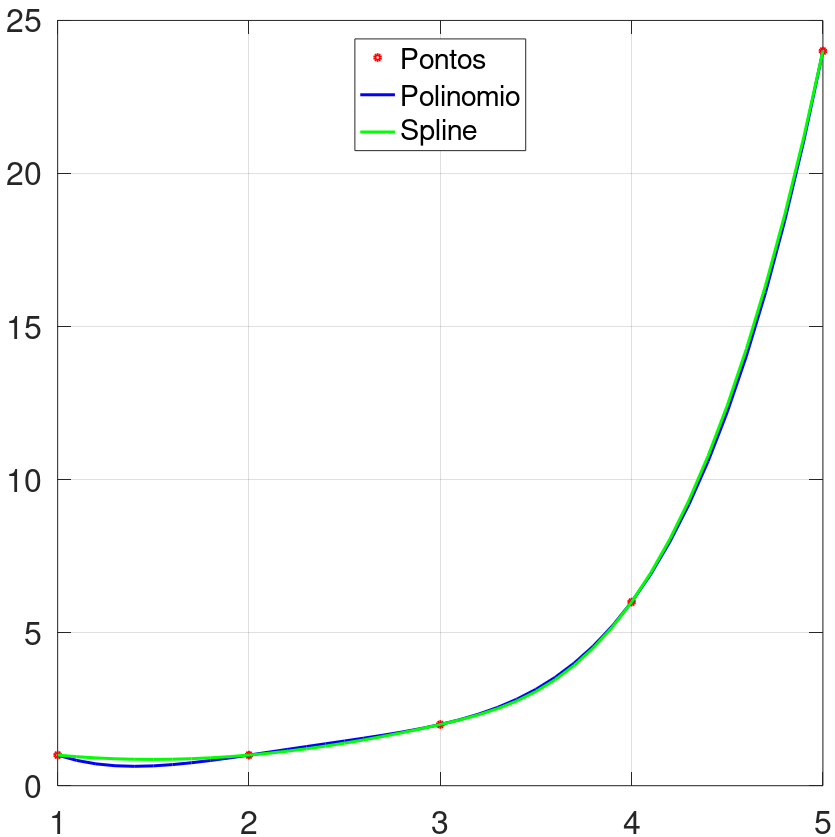
\includegraphics[width = 6cm]{polinomio.png}
                    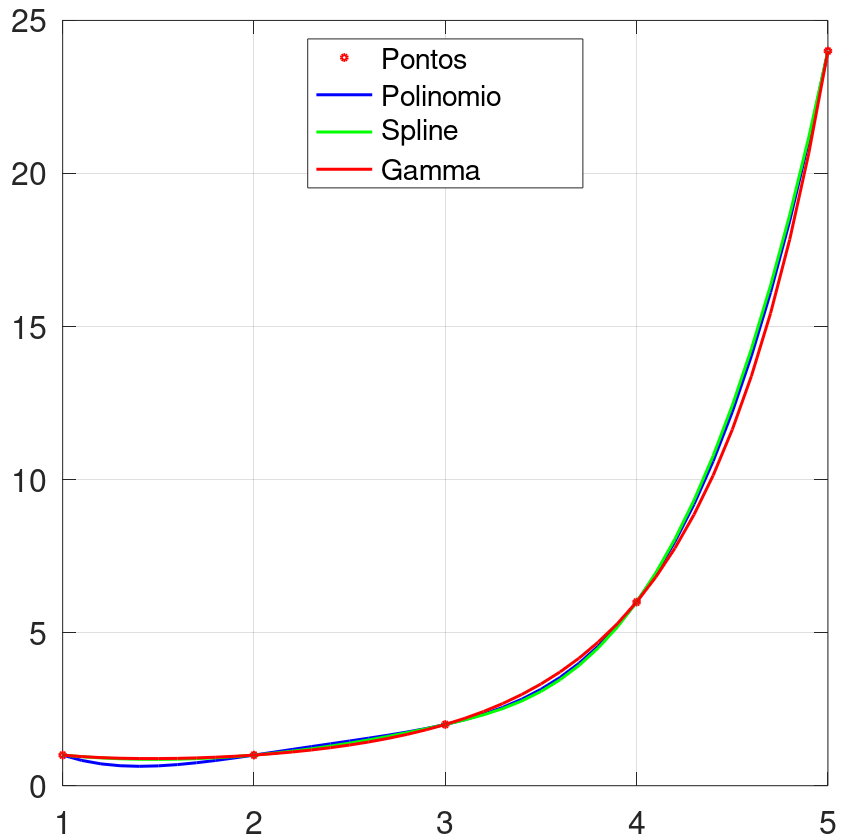
\includegraphics[width = 6.05cm]{polinomio1.png}
                    \centering
                \end{figure}
\newpage

            \paragraph{Intervalo $[1,5]$}Nota-se, através da inspeção visual, que a distância, consequentemente o erro, entre \texttt{Gamma} e a \textbf{Splice Cúbica}, no intervalo $[1,3]$, é menor. Entretanto, a distância entre \textbf{Gamma} e o \textbf{Polinômio}, no intervalo $[3,5]$, é menor. Ambas representam boas aproximações, a \textbf{Splice Cúbica} será superior por apresentar muito pouco erro no intervalo $[1,3]$.
                \begin{figure}[h]
                    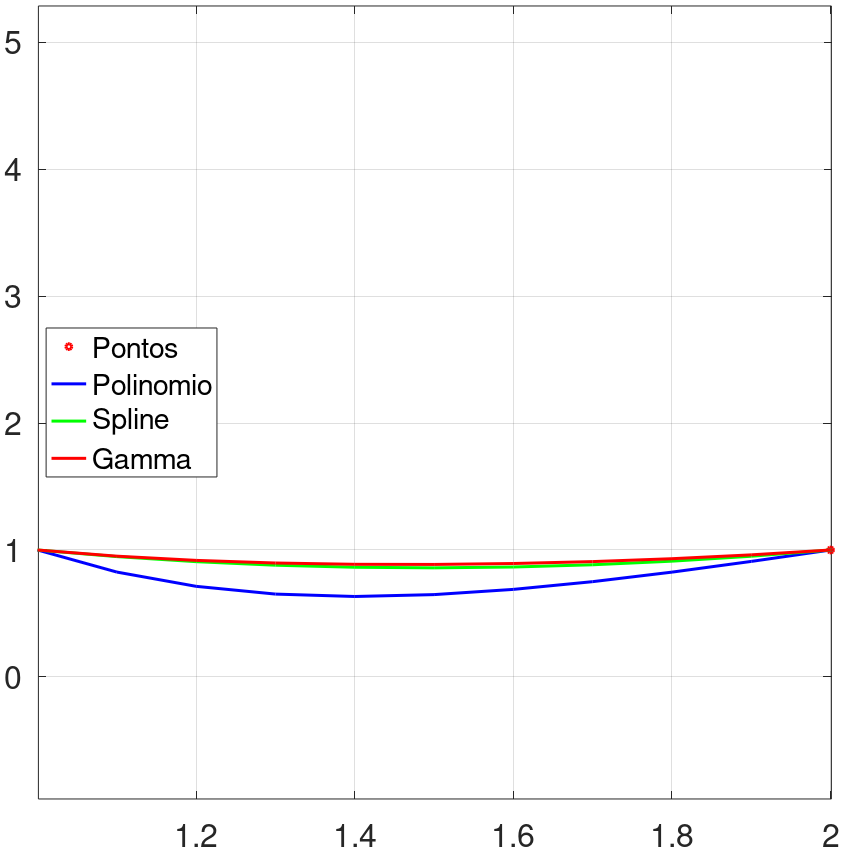
\includegraphics[width = 4cm]{zoom1.png}
                    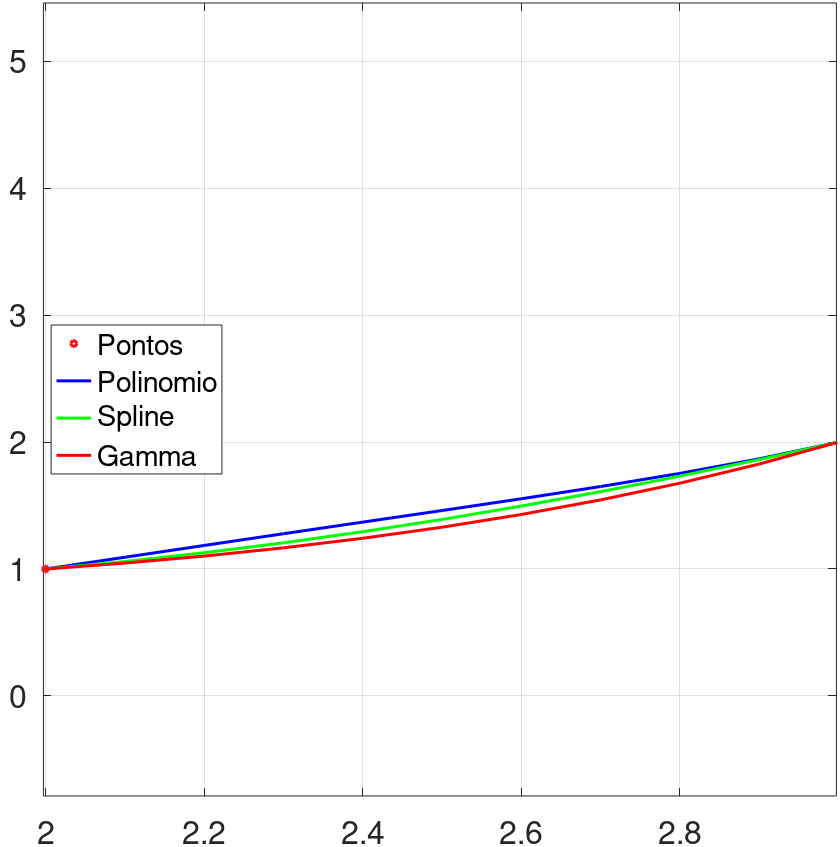
\includegraphics[width = 4cm]{zoom2.png}
                    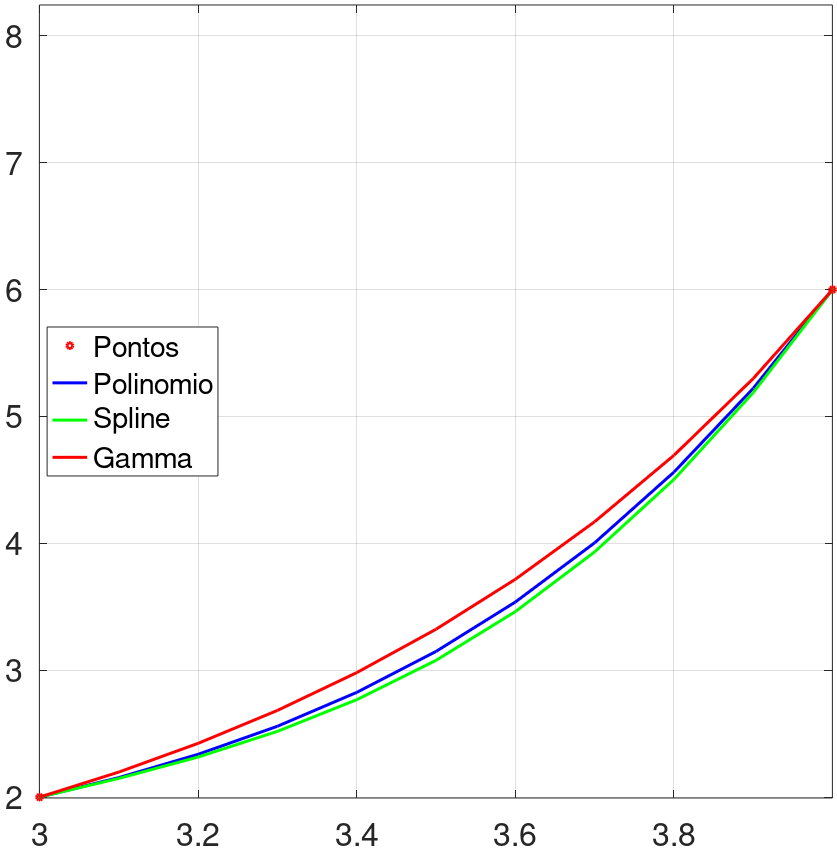
\includegraphics[width = 4cm]{zoom3.png}
                    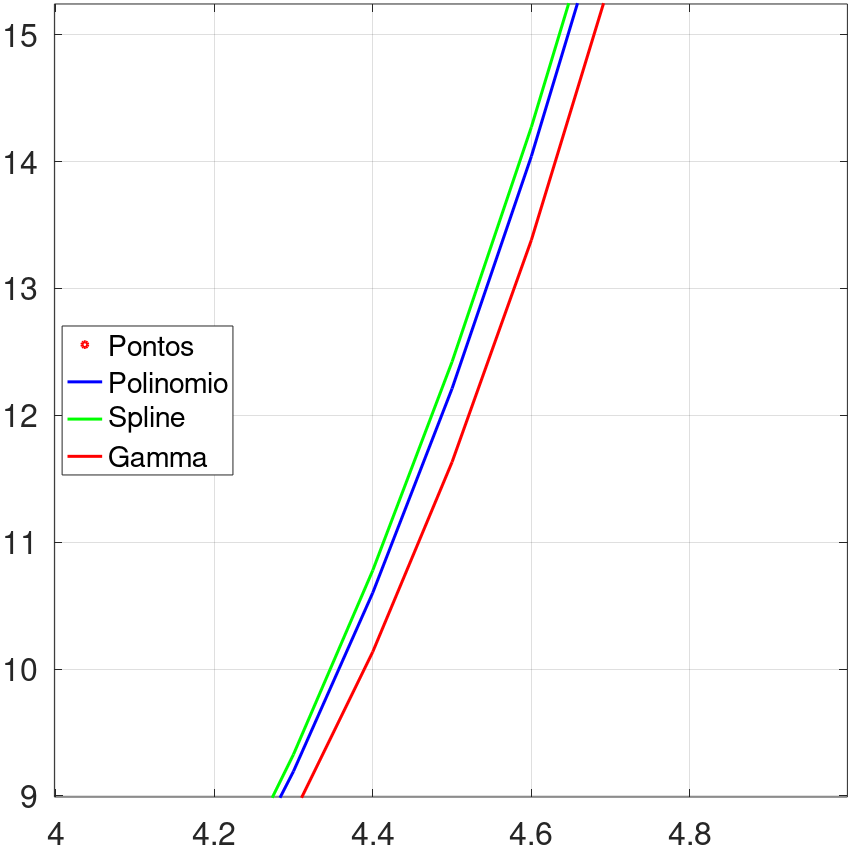
\includegraphics[width = 4cm]{zoom4.png}
                    \centering
                \end{figure}
                \paragraph{Intervalo $[1,2]$}A \textbf{Splice Cúbica} melhor aproxima a função \texttt{Gamma} no intervalo $[1,2]$. Nota-se que esta aproximação possui comportamento mais estável e suave, visto que está definida por partes. Isso garante maior precisão e menor sucessão ao \textbf{Efeito de Runge}.
                \begin{figure}[h]
                    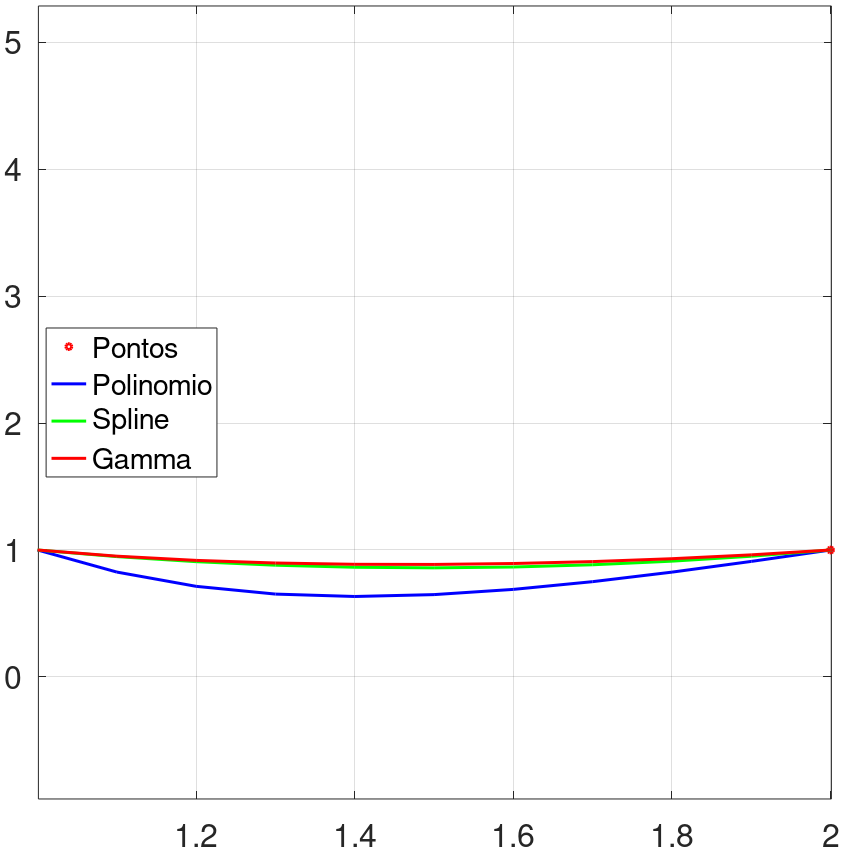
\includegraphics[width = 6cm]{zoom1.png}
                    \centering
                \end{figure}
\newpage

        \subsection{Códigos}
        \begin{scriptsize}
            \myStyle
            \lstinputlisting{CoeficientesNewton.m}
            \lstinputlisting{AT7_2.m}
        \end{scriptsize}
\newpage
\end{document}